\documentclass[12pt,letterpaper]{exam}
\usepackage[lmargin=1in,rmargin=1in,tmargin=1in,bmargin=1in]{geometry}
\usepackage{../style/exams}

% -------------------
% Course & Exam Information
% -------------------
\newcommand{\course}{MATH 142: Exam 1}
\newcommand{\term}{Fall ---\textsubscript{\textsubscript{1}} 2025}
\newcommand{\examdate}{09/23/2025}
\newcommand{\timelimit}{75 Minutes}

\setbool{hideans}{true} % Student: True; Instructor: False

\newcommand{\boxseven}[4]{%
	\draw[thick] (0,0) -- (4,0) -- (4,4) -- (0,4) -- (0,0);
	\draw[thick] (0,2) -- (4,2);
	\draw[thick] (2,0) -- (2,4);
	% '7'
	\draw[line width=0.03cm] (1.7,2.2) -- (2.3,2.2) -- (1.7,1.6);
	% Entries
	\node at (1,3) {$#1$};	% u
	\node at (3,1) {$#2$};	% dv
	\node at (1,1) {$#3$};	% du
	\node at (3,3) {$#4$};	% v
}


\usetikzlibrary{calc}
\usepackage{booktabs}
\tikzset{Arrow Style/.style={text=black, font=\boldmath}}
\newcommand{\tikzmark}[1]{%
    \tikz[overlay, remember picture, baseline] \node (#1) {};%
}
\newcommand*{\XShift}{0.5em}
\newcommand*{\YShift}{0.5ex}
\NewDocumentCommand{\DrawArrow}{s O{} m m m}{%
    \begin{tikzpicture}[overlay,remember picture]
        \draw[->, thick, Arrow Style, #2] 
                ($(#3.west)+(\XShift,\YShift)$) -- 
                ($(#4.east)+(-\XShift,\YShift)$)
        node [midway,above] {#5};
    \end{tikzpicture}%
}

\usepackage{cancel}

% -------------------
% Content
% -------------------
\begin{document}

\examtitle
\instructions{Write your name on the appropriate line on the exam cover sheet. This exam contains \numpages\ pages (including this cover page) and \numquestions\ questions. Check that you have every page of the exam. Answer the questions in the spaces provided on the question sheets. Be sure to answer every part of each question and show all your work. If you run out of room for an answer, continue on the back of the page --- being sure to indicate the problem number.
} 
\scores
\bottomline
\newpage


% -------------------
% Questions
% -------------------
\begin{questions}

% Question 1
\newpage
\question[15] Showing all your work, compute the following:
	\[
	\int \sin^3(4x) \cos^6(4x) \;dx
	\] \pspace

\vsol{\itshape This is a trigonometric integral because it is a product of powers of trig. functions. Observe that if we let $u= \sin(4x)$, then $du$ has a factor of cosine. This would leave an odd power of cosine left in the integrand and we can only replace even powers of cosine using the Pythagorean Identity. Therefore, we must choose $u= \cos(4x)$. But then\dots
	\[
	\begin{aligned}
	u&= \cos(4x) \\
	du&= -4\sin(4x) \;dx
	\end{aligned}
	\]
Recall that $\sin^2 \theta + \cos^2 \theta= 1$. Therefore, we know $\sin^2 \theta= 1 - \cos^2 \theta$. Using this identity in our integral and setting up our $u$-substitution, we have\dots
	\[
	\begin{aligned}
	\int \sin^3(4x) \cos^6(4x) \;dx&= \int \cos^6(4x) \sin^3(4x) \;dx \\[0.3cm]
	&= \int \cos^6(4x) \sin^2(4x) \cdot \sin(4x) \;dx \\[0.3cm]
	&= -\dfrac{1}{4} \int \cos^6(4x) \sin^2(4x) \cdot -4\sin(4x) \;dx \\[0.3cm]
	&= -\dfrac{1}{4} \int \cos^6(4x) \big(1 - \cos^2(4x) \big) \cdot -4\sin(4x) \;dx \\[0.3cm]
	&= -\dfrac{1}{4} \int u^6 (1 - u^2) \;du \\[0.3cm]
	&= -\dfrac{1}{4} \int (u^6 - u^8) \;du \\[0.3cm]
	&= -\dfrac{1}{4} \left( \dfrac{u^7}{7} - \dfrac{u^8}{8} \right) + C \\[0.3cm]
	&= \boxed{-\dfrac{1}{4} \left( \dfrac{\cos^7(4x)}{7} - \dfrac{\cos^8(4x)}{8} \right) + C} \\[0.3cm]
	&= \dfrac{\cos^7(4x)}{224}\, \big( 7\cos(4x) - 8 \big) + C
	\end{aligned}
	\]
}



% Question 2
\newpage
\question[15] Showing all your work, compute the following:
	\[
	\int x^3 \sin(2x) \;dx
	\] \pspace

\vsol{\itshape This is a tabular integration-by-parts because the integrand is a product of a polynomial and a trigonometric function. Using LIATE, we choose $u= x^3$, so that $dv= \sin(2x)$. 
	\[
	\begin{array}{c @{\hspace*{1.3cm}} c} \toprule
	u & dv \\ \cmidrule(lr){1-2}
	x^3 \tikzmark{Left 1} & \tikzmark{Right 1} \sin(2x) \\[0.3cm]
	3x^2 \tikzmark{Left 2} & \tikzmark{Right 2} -\dfrac{\cos(2x)}{2} \\[0.3cm]
	6x \tikzmark{Left 3} & \tikzmark{Right 3} -\dfrac{\sin(2x)}{4} \\[0.3cm]
	6 \tikzmark{Left 4} & \tikzmark{Right 4} \dfrac{\cos(2x)}{8} \\[0.3cm]
	0 \tikzmark{Left 5} & \tikzmark{Right 5} \dfrac{\sin(2x)}{16}
	
	\DrawArrow{Left 1}{Right 2}{+}
	\DrawArrow{Left 2}{Right 3}{--}
	\DrawArrow{Left 3}{Right 4}{+}
	\DrawArrow{Left 4}{Right 5}{--}
	\end{array}
	\]
Therefore, we have\dots
	\[
	\begin{aligned}
	\int x^3 \sin(2x) \;dx&= \boxed{-\dfrac{1}{2}\, x^3 \cos(2x) + \dfrac{3}{4}\, x^2 \sin(2x) + \dfrac{6}{8}\, x \cos(2x) - \dfrac{6}{16} \, \sin(2x) + C} \\[0.3cm]
	&= -\dfrac{1}{2}\, x^3 \cos(2x) + \dfrac{3}{4}\, x^2 \sin(2x) + \dfrac{3}{4}\, x \cos(2x) - \dfrac{3}{8} \, \sin(2x) + C \\[0.3cm]
	&= -\dfrac{1}{8} \, \left( 4x^3 \cos(2x) - 6x^2 \sin(2x) - 6x \cos(2x) + 3 \sin(2x) \right) + C
	\end{aligned}
	\]
}



% Question 3
\newpage
\question[15] Showing all your work, compute the following:
	\[
	\int_0^1 \arcsin \theta \;d\theta
	\] 

\vsol{\itshape This is a `traditional' integration-by-parts. We choose $u= \arcsin \theta$ so that $dv= 1$. Therefore, we have\dots
	\[
	\begin{tikzpicture}[scale=0.99]
	\boxseven{\arcsin \theta}{1}{\dfrac{1}{\sqrt{1 - \theta^2}}}{\theta}
	\end{tikzpicture}
	\]
But then\dots
	\[
	\begin{aligned}
	\int_0^1 \arcsin \theta \;d\theta&= \theta \arcsin \theta \bigg|_0^1 - \int_0^1 \dfrac{\theta}{\sqrt{1 - \theta^2}} \;d\theta \\[0.1cm]
	&= \big(1 \arcsin(1) - 0 \arcsin(0) \big) - \int_0^1 \dfrac{\theta}{\sqrt{1 - \theta^2}} \;d\theta \\[0.1cm]
	&= \big( \frac{\pi}{2}  - 0 \big) - \int_0^1 \dfrac{\theta}{\sqrt{1 - \theta^2}} \;d\theta \\[0.1cm]
	&= \dfrac{\pi}{2} - \int_0^1 \dfrac{\theta}{\sqrt{1 - \theta^2}} \;d\theta
	\end{aligned}
	\] 
For the remaining integral, observe that if $u= 1 - \theta^2$, so that $du= -2\theta \;d\theta$. If $\theta= 0$, then $u= 1 - 0^2= 1$, and if $\theta= 1$ then $u= 1 - 1^2= 0$. But then\dots
	\[
	\begin{aligned}
	\int_0^1 \arcsin \theta \;d\theta&= \dfrac{\pi}{2} - \int_0^1 \dfrac{\theta}{\sqrt{1 - \theta^2}} \;d\theta \\
	&= \dfrac{\pi}{2} - \dfrac{1}{-2} \int_0^1 \dfrac{-2\theta}{\sqrt{1 - \theta^2}} \;d\theta \\
	&= \dfrac{\pi}{2} + \dfrac{1}{2} \int_1^0 \dfrac{du}{\sqrt{u}} \\
	&= \dfrac{\pi}{2} + \dfrac{1}{2} \cdot 2\sqrt{u} \,\bigg|_1^0 \\
	&= \dfrac{\pi}{2} + \sqrt{u} \,\bigg|_1^0 \\
	&= \dfrac{\pi}{2} + (0 - 1) \\
	&= \boxed{\dfrac{\pi}{2} - 1} \\
	&= \dfrac{\pi - 2}{2}
	\end{aligned}
	\]
}



% Question 4
\newpage
\question[15] Showing all your work, determine if the following integral converges or diverges. If it converges, compute its value. 
	\[
	\int_1^3 \dfrac{dx}{x - 2}
	\] \pspace

\vsol{\itshape Observe that $\dfrac{1}{x - 2}$ is not defined at $x= 2$ (it has an asymptote there), which is in the interval of integration. Therefore, this is an improper integral. We split this integral into two pieces, both of which must converge for the integral to converge. 
	\[
	\int_1^3 \dfrac{dx}{x - 2}= \int_1^2 \dfrac{dx}{x - 2} + \int_2^3 \dfrac{dx}{x - 2}
	\] \pspace
But then we have\dots
	\[
	\int_1^3 \dfrac{dx}{x - 2}:= \lim_{b \to 2^-} \int_1^b \dfrac{dx}{x - 2} + \lim_{b \to 2^+} \int_b^3 \dfrac{dx}{x - 2} 
	\] \pspace
Observe that\dots
	\[
	\int \dfrac{dx}{x - 2}= \ln|x - 2| + C
	\] \pspace
Therefore, we have\dots
	\[
	\begin{aligned}
	\lim_{b \to 2^-} \int_1^b \dfrac{dx}{x - 2}&= \lim_{b \to 2^-} \ln|x - 2| \;\bigg|_1^b= \lim_{b \to 2^-} \ln|b - 2| - \ln|-1|= \lim_{b \to 2^-} \ln|b - 2|= -\infty \\[0.3cm]
	\lim_{b \to 2^+} \int_b^3 \dfrac{dx}{x - 2}&= \lim_{b \to 2^+} \ln|x - 2| \;\bigg|_b^3= \ln|1| - \lim_{b \to 2^+} \ln|b - 2|= -\lim_{b \to 2^+} \ln|b - 2|= \infty
	\end{aligned}
	\] \pspace
Because neither of these integrals converge, the original integral does not converge. \pspace

\begin{center} Therefore, the integral $\ds\int_1^3 \dfrac{dx}{x - 2}$ is divergent. \end{center}
}



% Question 5
\newpage
\question[15] Showing all your work, compute the following:
	\[
	\int \dfrac{dx}{x^2 \sqrt{x^2 - 9}}
	\]

\vsol{\itshape We know from the Pythagorean Theorem that $a^2 + b^2= c^2$, which implies that $a^2= c^2 - b^2$. Taking $c^2= x^2$, i.e. $c= x$, and $b^2= 9$, i.e. $b= 3$, we have $a^2= c^2 - b^2= x^2 - 9$. This also shows that $a= \sqrt{x^2 - 9}$. There are two possible right triangles corresponding to these sides we could draw:
	\[
	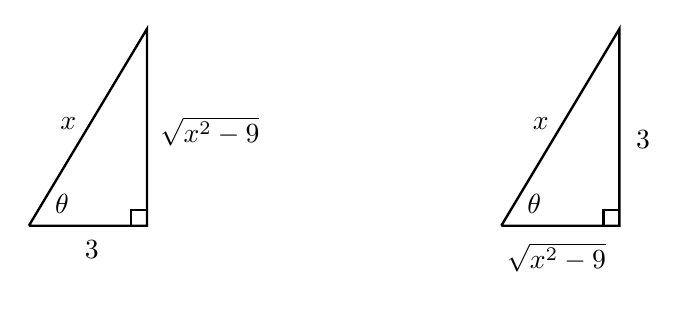
\begin{tikzpicture}
	\draw[line width=0.03cm] (0,0) -- (1.5,0) -- (1.5,2.5) -- (0,0);
	\draw[line width=0.03cm] (1.3,0) -- (1.3,0.2) -- (1.5,0.2);
	\node at (0.8,-0.3) {$3$};
	\node at (2.3,1.2) {$\sqrt{x^2 - 9}$};
	\node at (0.5,1.3) {$x$};
	\node at (0.42,0.28) {$\theta$};
	
	\tikzset{shift={(6,0)}};

	\draw[line width=0.03cm] (0,0) -- (1.5,0) -- (1.5,2.5) -- (0,0);
	\draw[line width=0.03cm] (1.3,0) -- (1.3,0.2) -- (1.5,0.2);
	\node at (1.8,1.1) {$3$};
	\node at (0.7,-0.4) {$\sqrt{x^2 - 9}$};
	\node at (0.5,1.3) {$x$};
	\node at (0.42,0.28) {$\theta$};
	\end{tikzpicture}
	\]
Using the right triangle on the left, we have $\cos \theta= \frac{3}{x}$, so that $x= \frac{3}{\cos \theta}= 3 \sec \theta$. But then $dx= 3 \sec \theta \tan \theta \;d\theta$. Because $x= 3 \sec \theta$, we know $x^2= 9 \sec^2 \theta$. Observe that $\tan \theta= \frac{\sqrt{x^2 - 9}}{3}$, so that $\sqrt{x^2 - 9}= 3 \tan \theta$. But then\dots
	\[
	\hspace{-1.2cm}\int \dfrac{dx}{x^2\sqrt{x^2 - 9}}= \int \dfrac{3 \sec \theta \tan \theta}{9 \sec^2 \theta \cdot 3 \tan \theta} \;d\theta= \int \dfrac{\cancel{3} \cancel{\sec \theta} \cancel{\tan \theta}}{9 \sec^{\cancel{2}} \theta \cdot \cancel{3} \cancel{\tan \theta}} \;d\theta= \int \dfrac{d\theta}{9 \sec \theta}= \dfrac{1}{9} \int \cos \theta \;d\theta= \dfrac{1}{9} \sin \theta + C
	\]
But from the right-triangle on the left, we know that $\sin \theta= \frac{\sqrt{x^2 - 9}}{x}$. Therefore, we have\dots
	\[
	\int \dfrac{dx}{x^2\sqrt{x^2 - 9}}= \dfrac{1}{9} \sin \theta + C= \boxed{\frac{\sqrt{x^2 - 9}}{9x} + C}
	\] \pspace
Alternatively, using the right triangle on the right, we have $\sin \theta= \frac{3}{x}$, so that $x= \frac{3}{\sin \theta}= 3 \csc \theta$. But then $dx= -3 \csc \theta \cot \theta$. Because $x= 3 \csc \theta$, we know $x^2= 9 \csc^2 \theta$. Observe that $\tan \theta= \frac{3}{\sqrt{x^2 - 9}}$, so that $\sqrt{x^2 - 9}= \frac{3}{\tan \theta}= 3 \cot \theta$. But then\dots
	\[
	\hspace{-2cm}\int \dfrac{dx}{x^2\sqrt{x^2 - 9}}= \int \dfrac{-3 \csc \theta \cot \theta}{9 \csc^2 \theta \cdot 3 \cot \theta} \;d\theta= \int \dfrac{\cancel{-3}^{-1} \cancel{\csc \theta} \cancel{\cot \theta}}{9 \csc^{\cancel{2}} \theta \cdot \cancel{3} \cancel{\cot \theta}} \;d\theta= \int \dfrac{-1}{9 \csc \theta} \;d\theta= -\dfrac{1}{9} \int \sin \theta \;d\theta= \dfrac{1}{9} \cos \theta + C
	\]
But from the right-triangle on the right, we know that $\cos\theta= \frac{\sqrt{x^2 - 9}}{x}$. Therefore, we have\dots
	\[
	\int \dfrac{dx}{\sqrt{x^2 - 9}}= \dfrac{1}{9} \cos \theta + C= \boxed{\frac{\sqrt{x^2 - 9}}{9x} + C}
	\]
}



% Question 6
\newpage
\question[15] Showing all your work, compute the following:
	\[
	\int \dfrac{-5x^2 + x - 3}{x^3 + x} \;dx
	\] \pspace

\vsol{\itshape Because the integrand is a rational function, this is a partial fraction integral. The degree of the numerator is already strictly less than that of the denominator. We need now factor the denominator completely. But $x^3 + x= x(x^2 + 1)$. Therefore, the partial fraction decomposition of the integrand has the following form:
	\[
	\dfrac{-5x^2 + x - 3}{x^3 + x}= \dfrac{A}{x} + \dfrac{Bx + C}{x^2 + 1}
	\]
Using the original common denominator $x(x^2 + 1)$, we have\dots
	\[
	\begin{aligned}
	\dfrac{-5x^2 + x - 3}{x^3 + x}&= \dfrac{A}{x} + \dfrac{Bx + C}{x^2 + 1} \\[0.3cm]
	&= \dfrac{A(x^2 + 1) + x(Bx + C)}{x(x^2 + 1)} \\[0.3cm]
	&= \dfrac{Ax^2 + A + Bx^2 + Cx}{x(x^2 + 1)}
	\end{aligned}
	\]
Equating the numerators and relating coefficients, we have\dots \par
	\begin{table}[!ht]
	\centering
	\begin{tabular}{ll}
	$x^2 \colon$ & $-5= A + B$ \\
	$x \colon$ & $1= C$ \\
	$1 \colon$ & $-3= A$
	\end{tabular}
	\end{table} \par
Because $A= -3$ and $-5= A + B$, we know that $B= -5 - A= -5 - (-3)= -2$. Therefore, $A= -3$, $B= -2$, and $C= 1$. But then\dots
	\[
	\begin{aligned}
	\int \dfrac{-5x^2 + x - 3}{x^3 + x} \;dx&= \int \left( \dfrac{-3}{x} + \dfrac{-2x + 1}{x^2 + 1} \right) \;dx \\[0.3cm]
	&= \int \left( \dfrac{-3}{x} - \dfrac{2x}{x^2 + 1} + \dfrac{1}{x^2 + 1} \right) \;dx \\[0.3cm]
	&= \boxed{-3\ln|x| - \ln|x^2 + 1| + \arctan x + K}
	\end{aligned}
	\]
}



% Question 7
\newpage
\question[15] Showing all your work, compute the following:
	\[
	\int \sin(3x) \cos(x) \;dx
	\] 

\vsol{\vspace{-0.1cm}\footnotesize\itshape Because the integrand is a product of trigonometric functions with differing arguments, we may suspect that this is a `looping' integration-by-parts, i.e. that we can use a `modified tabular' approach. Indeed, we can integrate this using this approach. We take $u= \sin 3x$ and $dv= \cos x$. We then have\dots 
	\[
	\begin{array}{c @{\hspace*{1.3cm}} c} \toprule
	u & dv \\ \cmidrule(lr){1-2}
	\sin(3x) \tikzmark{Left 1} & \tikzmark{Right 1} \cos(x) \\[0.5cm]
	3\cos(3x) \tikzmark{Left 2} & \tikzmark{Right 2} \sin(x) \\[0.3cm]
	-9\sin(3x) \tikzmark{Left 3}  & \tikzmark{Right 3} -\cos(x)
	
	\DrawArrow{Left 1}{Right 2}{+}
	\DrawArrow{Left 2}{Right 3}{--}
	\DrawArrow{Left 3}{Right 3}{\!\!\!\!\!$\phantom{}_{\genfrac{}{}{0pt}{}{}{+}}$}
	\end{array}
	\] 
But then we have\dots
	\[
	\begin{gathered}
	\int \sin(3x) \cos(x) \;dx= \sin(x) \sin(3x) + 3 \cos(x) \cos(3x) + \int 9 \sin(3x) \cos(x) \;dx \\[0.3cm]
	\int \sin(3x) \cos(x) \;dx= \sin(x) \sin(3x) + 3 \cos(x) \cos(3x) + 9 \int \sin(3x) \cos(x) \;dx \\[0.3cm]
	-8\int \sin(3x) \cos(x) \;dx= \sin(x) \sin(3x) + 3 \cos(x) \cos(3x) \\[0.3cm]
	\boxed{\int \sin(3x) \cos(x) \;dx= \dfrac{\sin(x) \sin(3x) + 3 \cos(x) \cos(3x)}{-8} + C}
	\end{gathered}
	\]
Of course, we instead could have chosen $u= \cos x$ and $dv= \sin(3x)$. In this case, we would have\dots
	\[
	\begin{array}{c @{\hspace*{1.3cm}} c} \toprule
	u & dv \\ \cmidrule(lr){1-2}
	\cos(x) \tikzmark{Left 1} & \tikzmark{Right 1} \sin(3x) \\[0.5cm]
	-\sin(x) \tikzmark{Left 2} & \tikzmark{Right 2} -\frac{1}{3}\,\cos(3x) \\[0.3cm]
	-\cos(x) \tikzmark{Left 3}  & \tikzmark{Right 3} -\frac{1}{9}\,\sin(3x)
	
	\DrawArrow{Left 1}{Right 2}{+}
	\DrawArrow{Left 2}{Right 3}{--}
	\DrawArrow{Left 3}{Right 3}{\!\!\!\!\!$\phantom{}_{\genfrac{}{}{0pt}{}{}{+}}$}
	\end{array}
	\] 
But then\dots
	\[
	\begin{gathered}
	\int \sin(3x) \cos(x) \;dx= -\frac{1}{3}\, \cos(x) \cos(3x) - \frac{1}{9} \sin(x) \sin(3x) + \int \frac{1}{9}\, \sin(3x) \cos(x) \;dx \\[0.3cm]
	\int \sin(3x) \cos(x) \;dx= -\frac{1}{3}\, \cos(x) \cos(3x) - \frac{1}{9} \sin(x) \sin(3x) + \frac{1}{9} \int \sin(3x) \cos(x) \;dx \\[0.3cm]
	\frac{8}{9} \int \sin(3x) \cos(x) \;dx= -\frac{1}{3}\, \cos(x) \cos(3x) - \frac{1}{9} \sin(x) \sin(3x) \\[0.3cm]
	\boxed{\int \sin(3x) \cos(x) \;dx= \frac{9}{8} \,\big(-\tfrac{1}{3}\, \cos(x) \cos(3x) - \tfrac{1}{9} \sin(x) \sin(3x) \big) + C} \\[0.3cm]
	\int \sin(3x) \cos(x) \;dx= \dfrac{-9\big(\tfrac{1}{3}\, \cos(x) \cos(3x) + \tfrac{1}{9} \sin(x) \sin(3x) \big)}{8} + C \\[0.3cm]
	\int \sin(3x) \cos(x) \;dx= \dfrac{\sin(x) \sin(3x) + 3 \cos(x) \cos(3x)}{-8} + C
	\end{gathered}
	\]
}

\vsol{
\newpage
{
\thispagestyle{empty}
\footnotesize \itshape
Alternatively, we can use the product-to-sum rule:
	\[
	\sin \theta \cos \phi= \dfrac{\sin(\theta + \phi) + \sin(\theta - \phi)}{2}
	\]
We have $\theta= 3x$ and $\phi= x$. Therefore, we have\dots
	\[
	\begin{gathered}
	\int \sin(3x) \cos(x) \;dx \\[0.3cm]
	\int \dfrac{\sin(3x + x) + \sin(3x - x)}{2} \;dx \\[0.3cm]
	\dfrac{1}{2} \int \big( \sin(4x) + \sin(2x) \big) \;dx \\[0.3cm]
	\boxed{\dfrac{1}{2} \left[ -\dfrac{\cos(4x)}{4} - \dfrac{\cos(2x)}{2} \right] + C} \\[0.3cm]
	\dfrac{1}{2} \cdot -\dfrac{1}{4} \big( \cos(4x) + 2 \cos(2x) \big) + C \\[0.3cm]
	\dfrac{\cos(4x) + 2 \cos(2x)}{-8} + C
	\end{gathered}
	\]
\setcounter{page}{8}
}
}
	
\end{questions}
\end{document}